\documentclass[a4paper]{report}

\usepackage{ae,lmodern} % ou seulement l'un, ou l'autre, ou times etc.
\usepackage[francais]{babel}
\usepackage[utf8]{inputenc}
\usepackage[T1]{fontenc}
\usepackage{lipsum}% for dummy text
%\usepackage{multicol}% for multiple columns
\usepackage{listings}
\usepackage[dvipsnames]{xcolor}
\usepackage{graphicx}
\usepackage{palatino}
\usepackage{hyperref}
\usepackage[margin=2cm]{geometry}
\usepackage{makecell}
\usepackage{adjustbox}
\usepackage{caption}
\usepackage{subcaption}
%\usepackage{dirtree}

\definecolor{warning}{rgb}{1.0, 0.5, 0}

\title{\huge{Modèle d'un projet django}\\~\\
	Documentation de la partie serveur}

\author{Arezki ABERKANE\\a.aberkane@audensiel.fr}
\date{\today}

\begin{document}
	\maketitle
	\tableofcontents
\newpage
	
%\lstset{
%	string=[s]{"}{"},
%	stringstyle=\color{blue},
%	comment=[l]{:},
%	commentstyle=\color{black},
%	inputencoding=utf8
%}
	
%\part{partie}	-1
%\chapter{chapitre}	0
%\section{section}	1
%\subsection{sous-section}	2
%\subsubsection{sous-sous-section}	3
%\paragraph{paragraphe}	4
%\subparagraph{sous-paragraphe}	5


	
\part{Documentation}

\chapter{Manuel utilisateur}
\label{chap:manual}


\section{Plan du site et navigation}

La barre de navigation est située en haut et à gauche de chaque page du site et permet d'accéder rapidement à ses fonctions principales : Tableau de bord~\ref{sec:dashboard}, Visualisation des données~\ref{sec:graphics}, gestion des \emph{Kube}~\ref{sec:kube}, lancement d'analyses~\ref{sec:analyses}, et gestion des données~\ref{sec:datasets}.\\

Ces fonctions principales sont complétées par des icônes situées à droite de la barre supérieure :
\begin{description}
	\item[Manuel] Donne accès au manuel utilisateur~\ref{subsec:manual}
	\item[Tickets] derniers tickets ouverts~\ref{subsec:support}
	\item[Messages] derniers messages reçus~\ref{subsec:messages}
	\item[Tâches] dernières analyses lancées~\ref{subsec:last_tasks}
	\item[Notifications] dernières notifications reçues~\ref{subsec:notifications}
	\item[Menu utilisateur] Fonctions utilisateur
	\begin{description}
		\item[Profil] Modifier son profil utilisateur~\ref{subsec:profil}
		\item[Paramètres] Paramètres de l'interface graphique % TODO ~\ref{subsec:paramètres}
		\item[Déconnexion] déconnecte la session en cours
	\end{description}
\end{description}

\begin{figure}[h]
	\begin{tabular}[b]{p{9cm}}
		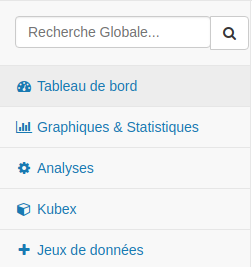
\includegraphics[width=0.5\textwidth]{images/leftNavig.png}\\
		\subcaption{\label{fig:leftnav} Barre de navigation}
\end{tabular}
\begin{tabular}[b]{p{9cm}}
	
\includegraphics[width=0.5\textwidth]{images/upNavig.png}\\
	\subcaption{\label{fig:upnav} Onglets de navigation}\\
	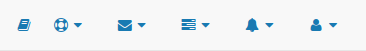
\includegraphics[width=0.5\textwidth]{images/upMenu.png}\\
	\subcaption{\label{fig:upmenu} Menu général}
\end{tabular}
\caption{\label{fig:base} Accès rapides présents sur toutes les pages}
\end{figure}
\newpage
\section{Tableau de bord}
\label{sec:dashboard}
Le tableau de bord est la page principale d'informations de l'interface Kubex, et également la première à s'ouvrir après s'être authentifié. Il contient de nombreux liens rapides et informations utiles qui permettent d'effectuer un tour d'horizon rapide de l'état des systèmes Kubex connectés et de leurs données.

\begin{figure}[h]
	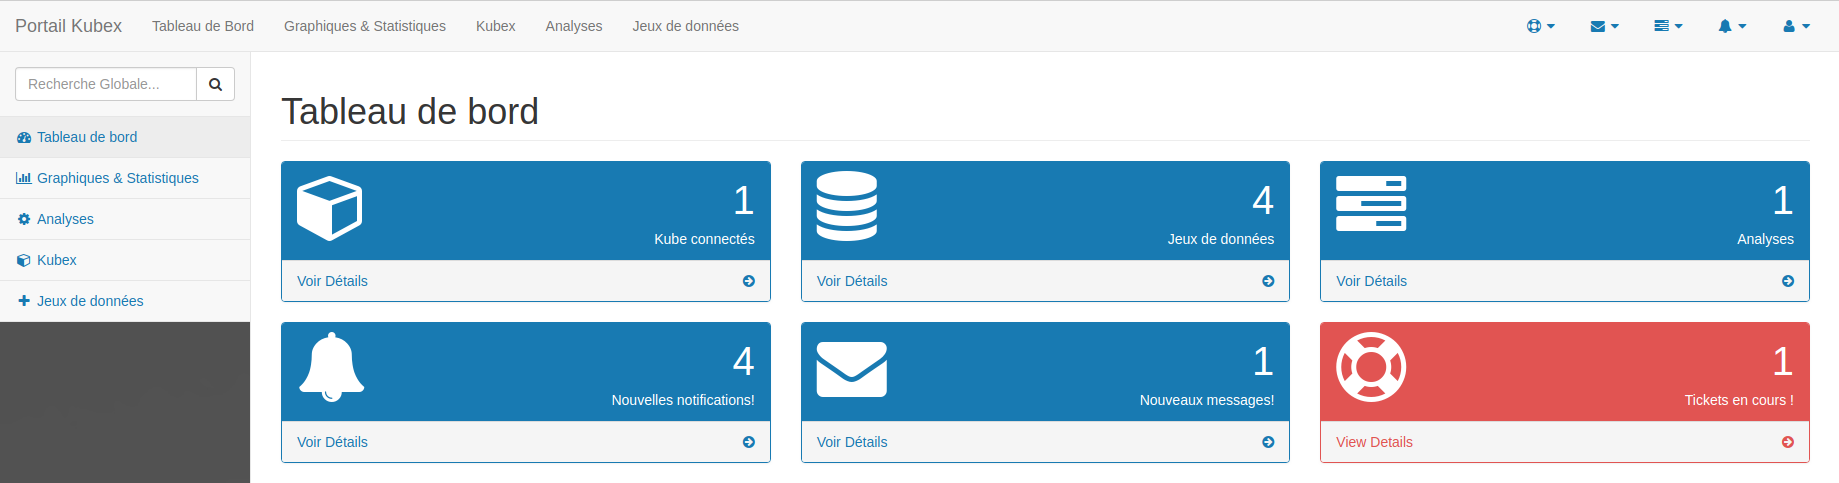
\includegraphics[width=\textwidth]{images/dashboard.png}
	\caption{\label{fig:dashboard} Tableau de bord}
\end{figure}

Le tableau de bord présente 6 différentes boites d'information rapide :

\begin{description}
	\item[Kube] Nombre de \emph{Kube} rattachés à l'utilisateur
	\item[Jeux de données] Jeux de données auxquels a accès l'utilisateur
	\item[Analyses] Analyses lancées par l'utilisateur
	\item[Notifications] Nouvelles notifications
	\item[Messages] Messages reçus non lus
	\item[Tickets] Tickets en cours de traitement
\end{description}

En cliquant sur la partie \emph{Plus de détails}, l'utilisateur accède directement à l'interface de gestion de la ressource concernée. De cette façon, il peut observer dès la page d'accueil l'état actuel du système et se rendre d'un simple clic sur les domaines où il souhaite agir.

\begin{figure}[h]
	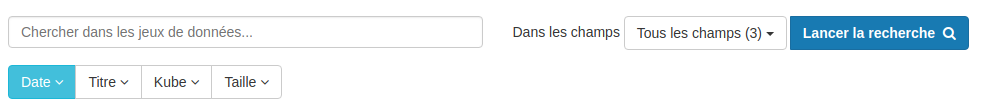
\includegraphics[width=\textwidth]{images/searchBar.png}
	\caption{\label{fig:search} Barre de recherche de jeu de données}
\end{figure}

Plus bas sur cette même page sont présentés les différents jeux de données accessibles accompagnés d'une barre de recherche et de tri, ce qui permet un accès rapide à leur édition ou au lancement d'analyses. Une frise chronologique des derniers événements permet également de résumer rapidement les évolutions survenues depuis la dernière connexion.

% to include ? maybe later...
%\begin{figure}[h]
%	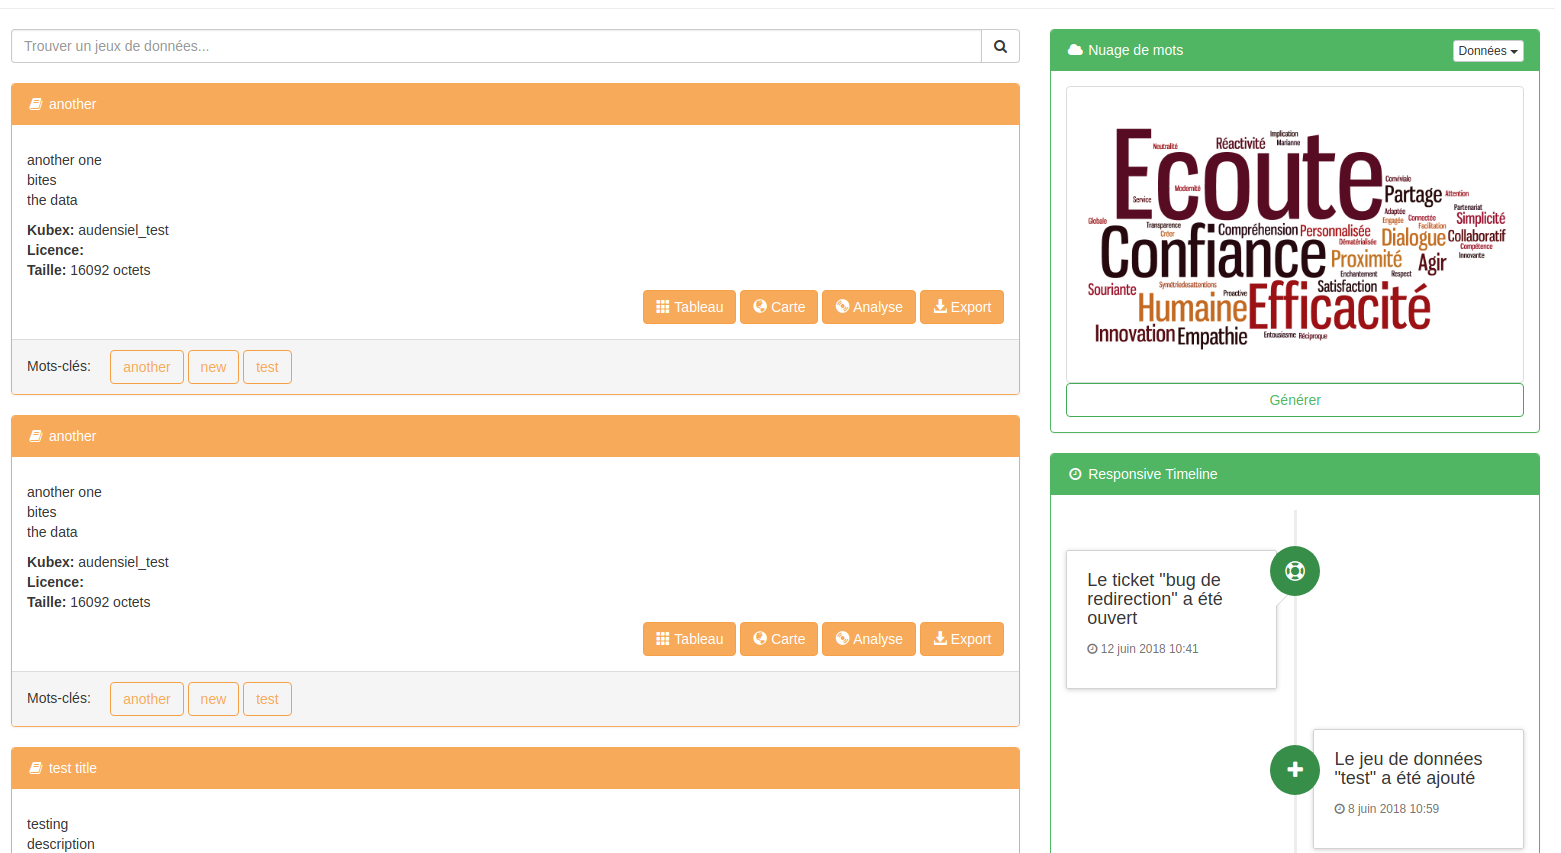
\includegraphics[width=\textwidth]{dashboard2.png}
%	\caption{\label{fig:dashboard2} Tableau de bord}
%\end{figure}



\newpage
\section{Visualisation des données}
\label{sec:graphics}

La première étape pour comprendre les jeux de données stockés dans le cloud est de les visualiser. Pour cela l'onglet de visualisation des données propose des outils diversifiés, adaptés à chaque type de données et de besoin. Ces visualisations restent ajustables dynamiquement même après affichage pour permettre une visualisation interactive des données.

\begin{figure}[h]
	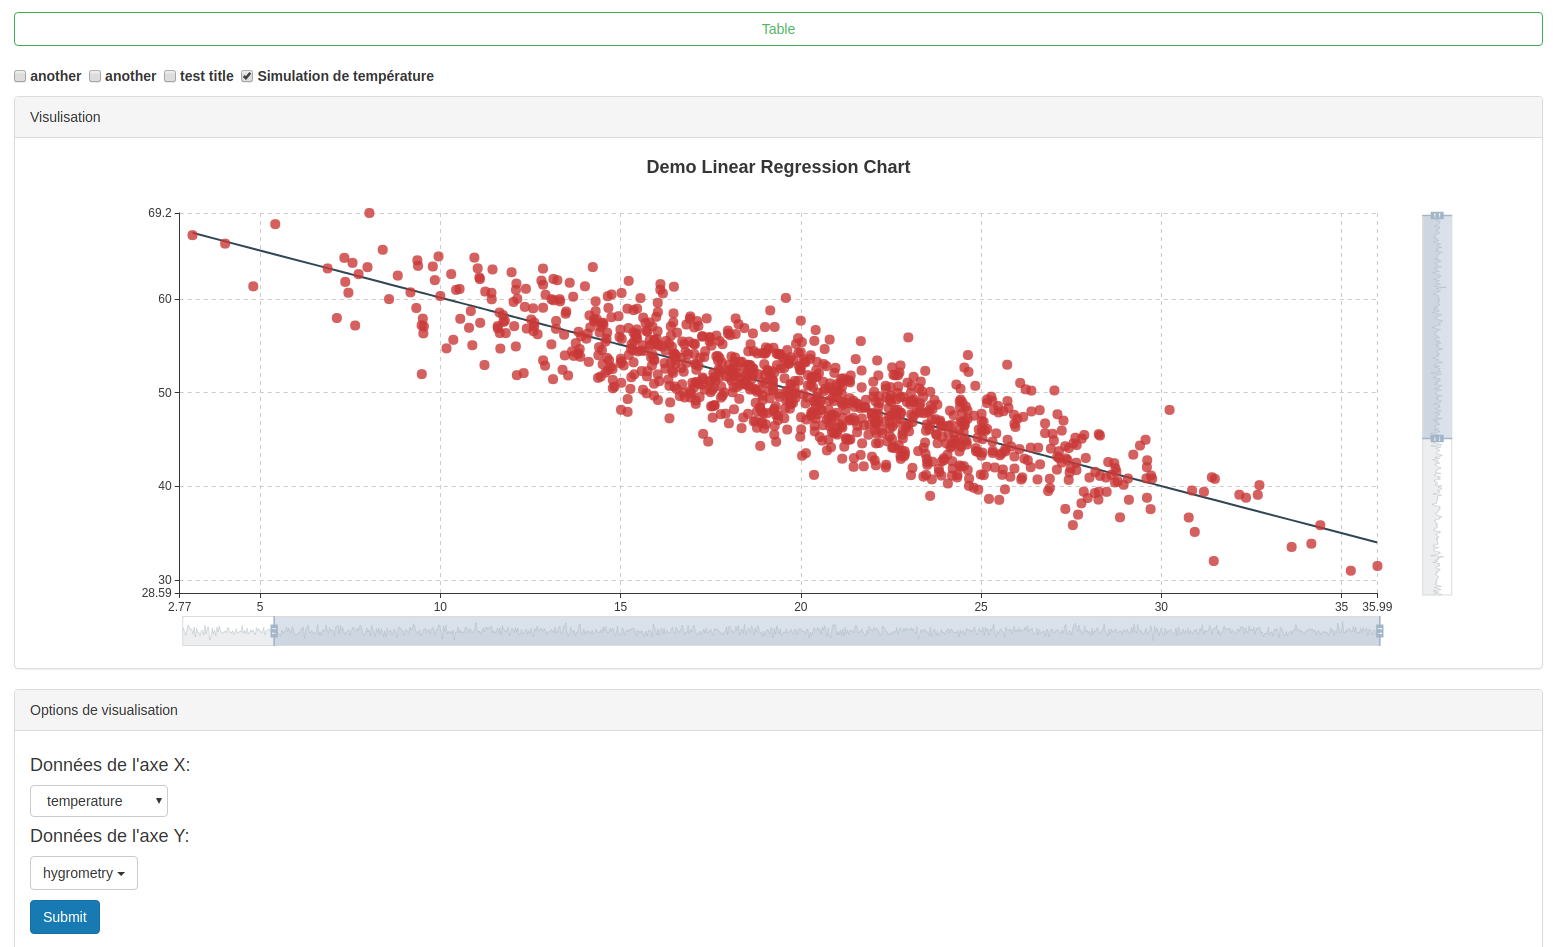
\includegraphics[width=\textwidth]{images/graphics.png}
	\caption{\label{fig:graphics} Visualisation de données}
\end{figure}

La première section permet de choisir le format de données du jeu de données à afficher, parmi des formats génériques très différents :

\begin{description}
	\item[Table] Tableau formaté de données numériques ou littéraire
	\item[Image] Collection d'images (incluant calques, filtres etc)
	\item[Audio] Sons et filtres associés
	\item[Video] Enregistrements vidéo (incluant calques, filtres, annotations etc)
\end{description}

La sélection de ce premier format permet de définir quel type de conteneur sera utilisé pour l'affichage, et de sélectionner les jeux de données parmi ceux dont le format correspond.
L'utilisateur sélectionne alors les jeux de données pour lesquels ils souhaite une visualisation parmi la liste générée dynamiquement, puis peut ensuite affiner l'affichage au moyen du panneau de contrôle.

Ce panneau contient en premier lieu le type de visualisation à afficher (par exemple pour un tableau de données le type de courbe ou graphique), puis les données à afficher au sein des jeux sélectionnés, la façon dont elles seront affichées, et divers paramètres d'affichage.

En appuyant sur le bouton \emph{Visualiser}, la visualisation souhaitée apparaît alors. Celle-ci reste modifiable soit au moyen du panneau de contrôle, soit directement en utilisant les outils pré-intégrés à celle-ci (zoom etc).
\newpage
\section{Kube}
\label{sec:kube}

Cette section permet de lister les \emph{Kube} auxquels un utilisateur a accès, renseignant les propriétés suivantes :

\begin{itemize}
	\item Nom du \emph{Kube}
	\item Numéro de série
	\item Utilisateurs
	\item Adresse IP
	\item Jeux de données associés
	\item Configuration (Administrateurs uniquement)
\end{itemize}
~\\
Pour les administrateurs des \emph{Box of Service} et Audensiel, il est également possible de gérer les \emph{Kube} à distance au moyen de cette interface, ce qui inclut leurs paramètres de fonctionnement mais aussi les capteurs et actionneurs auxquels ils sont reliés, les accès utilisateurs et la communication entre \emph{Box of Service} et le cloud.

\begin{figure}[h!]
	\begin{subfigure}[b]{0.5\textwidth}
		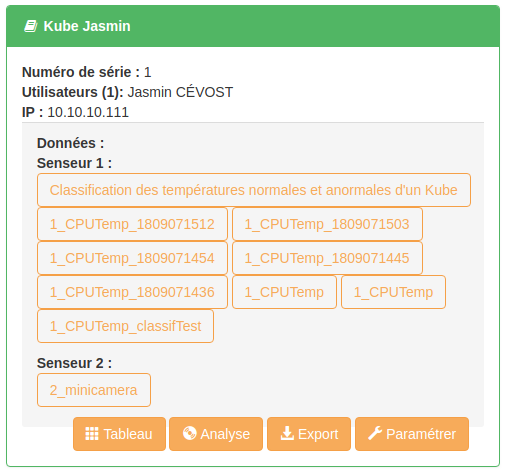
\includegraphics[width=\textwidth]{images/pageKubex2.png}
		\caption{\label{fig:kubeInfo} Gestion des \emph{Kube}}
	\end{subfigure}
	\begin{subfigure}[b]{0.5\textwidth}
		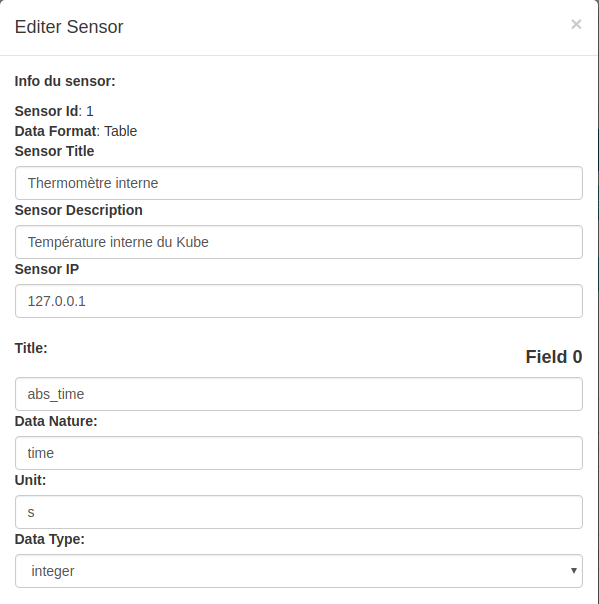
\includegraphics[width=\textwidth]{images/sensor_edit.png}
		\caption{\label{fig:sensorEdit} Edition de la configuration des capteurs}
	\end{subfigure}
	\caption{\label{fig:kubePage} Panneaux d'information et d'édition des \emph{Kube}}
\end{figure}

L'administrateur de la \emph{Box of Service} et les administrateurs Audensiel peuvent également voir et modifier directement la configuration des \emph{Kube} et capteurs au moyen d'un bouton \emph{Paramétrer} supplémentaire. Ce bouton ouvre la fenêtre modale \ref{fig:sensorEdit}.

Cette fenêtre permet de reconfigurer directement les capteurs sur le serveur; la nouvelle configuration sera propagée sous peu du serveur à la \emph{Box of Service}. Cette fonctionnalité peut être très efficace pour adapter la configuration de la BoS toute entière, cependant son utilisation doit faire le cas d'une extrême précaution, car toute fausse manipulation pourrait mettre complètement hors d'état la \emph{Box of Service}.

\newpage
\section{Analyses}
\label{sec:analyses}


Cet onglet permet à l'utilisateur de lancer des analyses sur tous les jeux de données auxquels il a accès, au moyen d'une liste d'algorithmes proposés.\\ 
L'utilisateur est ensuite invité à sélectionner les données d'entrée pour l'analyse depuis des listes générées à partir des jeux de données sélectionnés, de la même façon que pour la visualisation de données.\\

\begin{figure}[h!]
	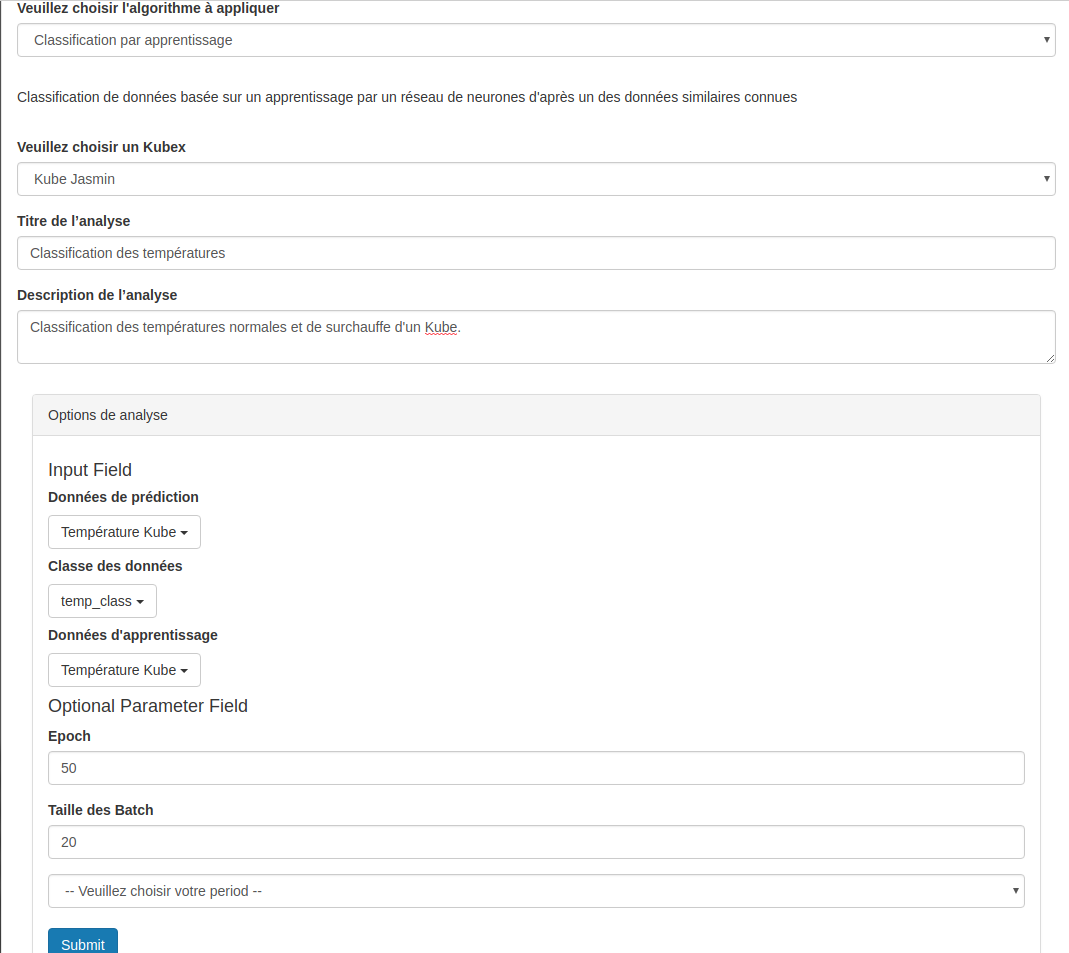
\includegraphics[width=\textwidth]{images/pageAnalyse.png}
	\caption{\label{fig:analyse} Formulaire de lancement d'analyses}
\end{figure}
~\\
Le formulaire ci-dessus s'affiche alors, invitant l'utilisateur à rattacher l'analyse à une \emph{Kube}, lui donner un titre et une description. Les champs de titre et de description serviront non seulement pour l'analyse, mais aussi pour les jeux de données qu'elle générera.\\
Les champs nécessaires aux données d'entrée et paramètres de l'algorithme sont alors générés automatiquement, l'utilisateur n'a alors plus qu'à sélectionner les entrées souhaitées. De plus, les paramètres sont remplis avec une valeur par défaut pour permettre aussi bien aux utilisateurs novices de lancer des analyses déjà paramétrées qu'aux utilisateurs expérimentés de personnaliser plus finement leurs analyses.

\newpage
\section{Jeux de données}
\label{sec:datasets}

Cet onglet permet de gérer les jeux de données générés par les \emph{Kube} auxquels l'utilisateur a accès. Chaque jeu de données est présenté sous la forme d'un panneau où figurent son titre, sa description, son format (tableau/image/son/vidéo), le système Kubex auquel il est rattaché, mais aussi sa taille et les mots-clés qui lui sont associés.
Il est possible de renommer les jeux de données, modifier leur description, ajouter des mots-clés, mais aussi ajouter de nouveaux jeux de données externes et les associer à un \emph{Kube} existant pour procéder à des analyses comparatives.

\begin{figure}[h!]
	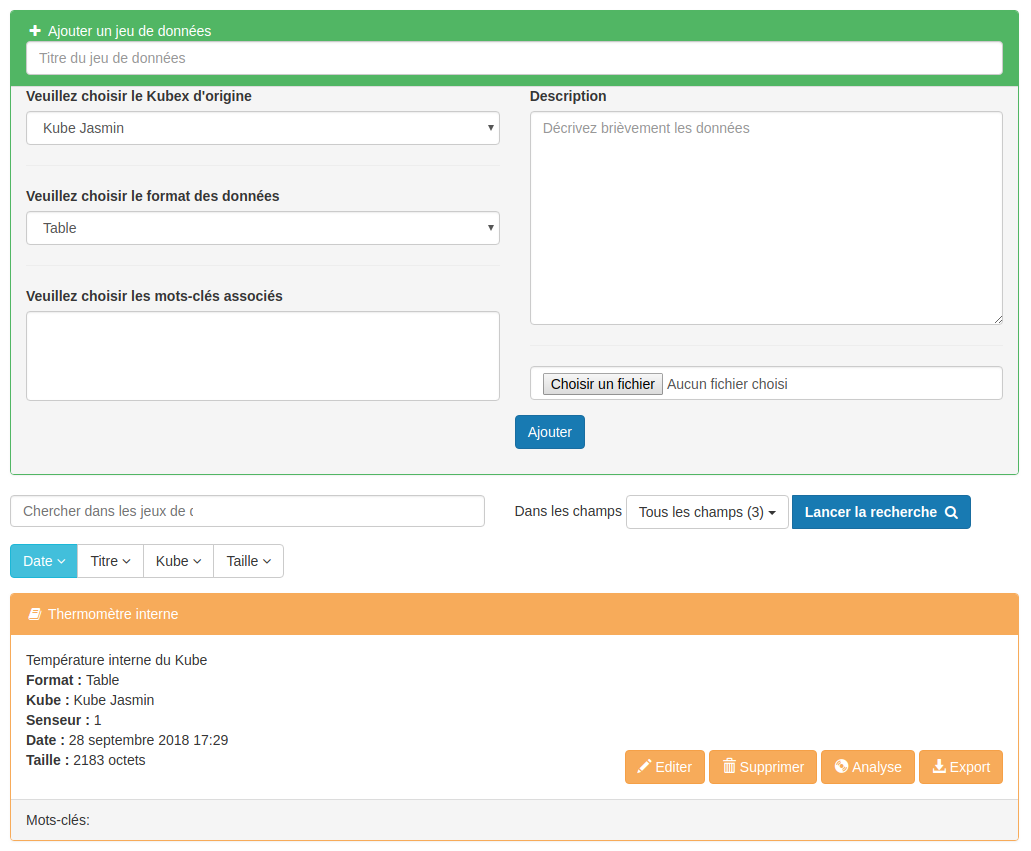
\includegraphics[width=\textwidth]{images/datasets.png}
	\caption{\label{fig:datasets} Ajout externe et modification des jeux de données}
\end{figure}
\newpage
\section{Autres fonctionnalités}

Cette section détaille les autres fonctionnalités accessoires de l'interface Kubex. Celles-ci sont accessibles depuis le menus de la barre supérieure et possèdent chacune une page qui leur est dédiée. Ces fonctionnalités supplémentaires ne son pas nécessaires à l'utilisation de l'interface Kubex, mais elles présentent cependant de nombreux services utiles pour les utilisateurs.

\subsection{Accès au manuel}
\label{subsec:manual}

Il est possible d'accéder à ce manuel utilisateur depuis la page de connexion ou depuis le menu situé en haut de chaque page, comme présenté ci-dessous :

\begin{figure}[h!]
	\centering
	
\includegraphics[width=0.5\textwidth]{images/loginManual.png}
	\caption{\label{fig:manual} Accès au manuel utilisateur depuis la page de connexion}
\end{figure}

\begin{figure}[h!]
	\centering
	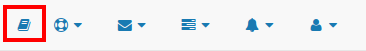
\includegraphics[width=0.5\textwidth]{images/menuManual.png}
	\caption{\label{fig:manual} Accès au manuel utilisateur depuis le menu}
\end{figure}

En cliquant sur ces liens, ce manuel sera directement envoyé à l'utilisateur au format PDF, pour être ensuite ouvert par le navigateur directement ou téléchargé pour être consulté localement.

\subsection{Support}
\label{subsec:support}

Le centre de support utilisateur est accessible depuis la liste des tickets en cours, soit en cliquant sur l'icône de bouée dans le menu, soit depuis le récapitulatif présenté dans le tableau de bord (voir ci-dessous).

\begin{figure}[h!]
	\centering
	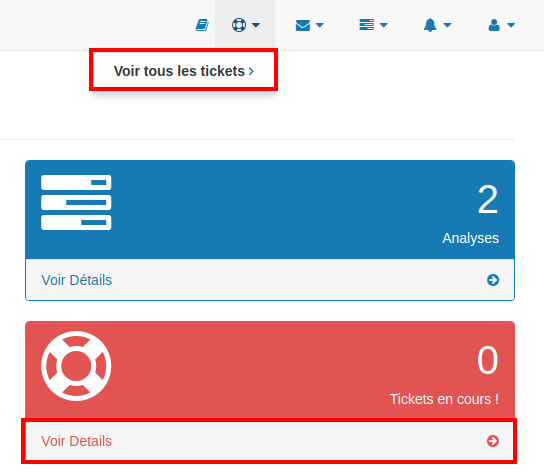
\includegraphics[width=0.5\textwidth]{images/accesSupport.png}
	\caption{\label{fig:accSupport} Accès au support utilisateur}
\end{figure}

Le support utilisateur se base principalement sur le système de tickets : quand un utilisateur souhaite faire une requête au support Kubex pour son compte ou un tiers, rencontre des difficultés, a remarqué un dysfonctionnement ou demande de nouvelles fonctionnalités, il peut créer un ticket dans cette section, qui sera assigné à un membre du support Kubex afin d'être suivi et résolu dans les plus brefs délais.\\

\begin{figure}[h]
	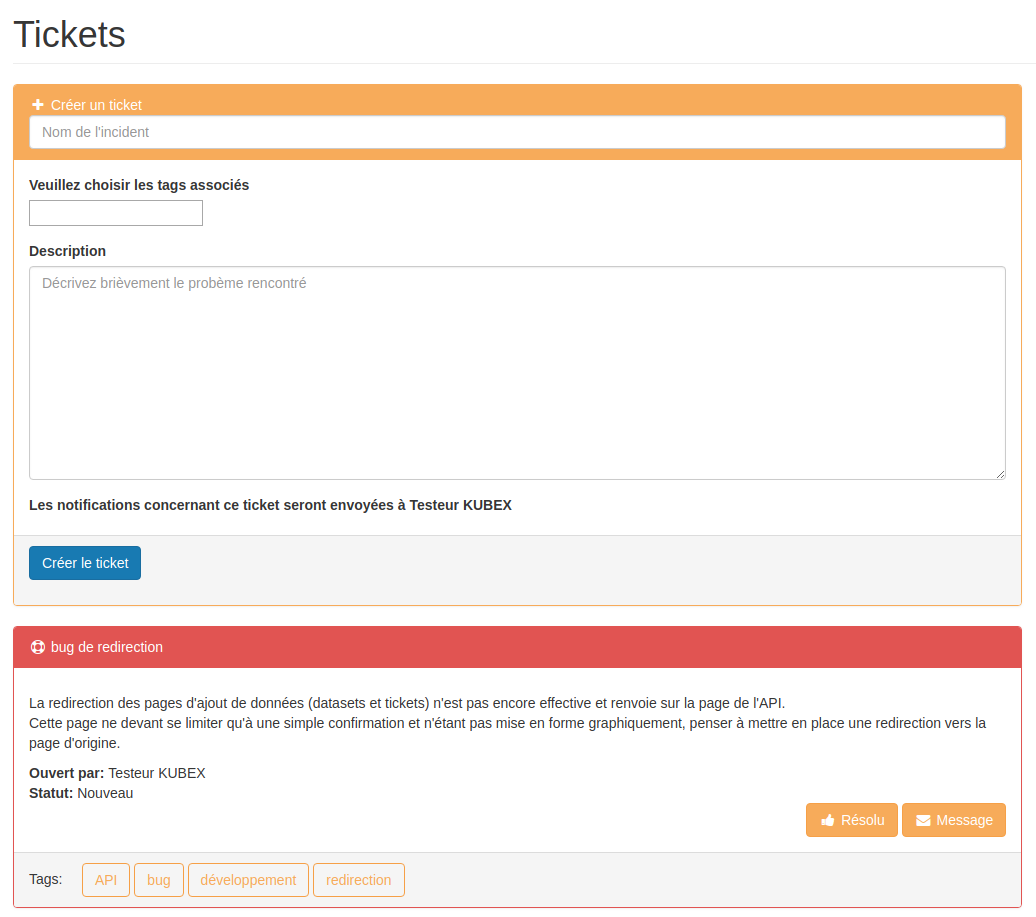
\includegraphics[width=\textwidth]{images/support.png}
	\caption{\label{fig:support} Centre de support utilisateur}
\end{figure}

Pour créer un ticket, il suffit de lui donner un titre clair, puis de décrire aussi précisément que possible la requête dans le champ "description" et éventuellement ajouter des tags représentant le type de requête et le domaine concerné pour qu'il soit assigné aux personnes adéquates le plus rapidement possible. En cliquant sur "Valider", le ticket sera alors automatiquement envoyé au staff Kubex dont une personne pourra alors le prendre en charge.
Pendant toute la période où le ticket sera ouvert, il sera possible de suivre son évolution sur cette même page, au moyen de plusieurs informations :

\begin{itemize}
	\item Titre
	\item Description
	\item Auteur
	\item Statut
	\begin{description}
		\item[Nouveau] Ticket nouvellement créé encore non assigné
		\item[Assigné] Ticket pris en charge par un membre du staff
		\item[En attente] Ticket en attente d'une action extérieure
		\item[Résolu] Ticket résolu et validé par son auteur
	\end{description}
	\item Responsable dans le staff
	\item Tags du ticket
	\item Actions sur le ticket
	\begin{itemize}
		\item Marquer comme résolu
		\item Envoyer un message au responsable
	\end{itemize}
\end{itemize}

\subsection{Messagerie}
\label{subsec:messages}

L'interface web Kubex propose également la possibilité d'échanger des messages entre les différents utilisateurs et administrateurs. Ceci permet de faciliter grandement la communication entre les acteurs au sein d'une \emph{Box of Service} et avec les administrateurs Kubex. Il suffit alors d'envoyer un simple message au moyen de cette interface à la personne de son choix pour communiquer de façon rapide et efficace au sujet de Kubex, que ce soit pour échanger à propos des résultats obtenus ou d'un  ticket en cours. Cette fonction est complémentaire à une boite mail classique est amenée à être reliée à l'adresse mail utilisateur dans le futur.

\begin{figure}[h]
	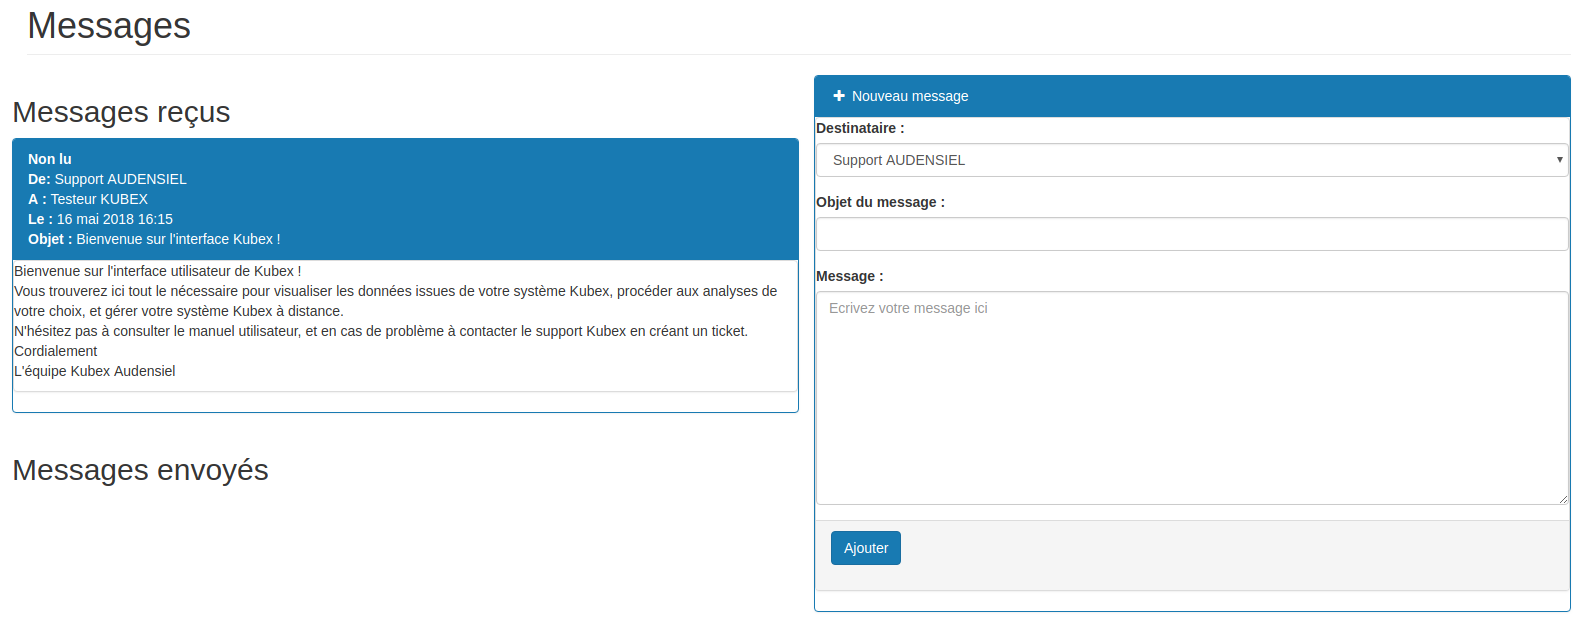
\includegraphics[width=\textwidth]{images/messages.png}
	\caption{\label{fig:messages} Messagerie Kubex}
\end{figure}

\subsection{Suivi des analyses}
\label{subsec:last_tasks}

Cette page permet d'afficher un le résumé des analyses en cours et passées. Celles-ci sont représentés au moyen de petits panneaux dont la couleur indique leur statut :

\begin{description}
	\item[bleu] En cours
	\item[vert] Terminée (avec succès)
	\item[rouge] En erreur
	\item[jaune] En pause (non implémenté)
\end{description}

\subsection{Notifications}
\label{subsec:notifications}

Cette page recense l'ensemble des notifications reçues par l'utilisateur. La couleur de celles-ci recense le type de notification et permet d'avoir un aperçu rapide du nombre d'erreurs et validations.

\begin{description}
	\item[bleu] Information générale, historique
	\item[vert] Confirmation, tâche effectuée avec succès
	\item[rouge] Erreur
	\item[jaune] Avertissement, message à lire
\end{description}

Une fois la notification lue, il est possible de la nettoyer d'un simple clic sur la croix pour qu'elle n'apparaisse plus, ou au contraire de la conserver pour plus tard.
\newpage
\subsection{Profil}
\label{subsec:profil}

Cette page permet à l'utilisateur de modifier ses informations personnelles, ainsi que son mot de passe. Il présente également les groupes dont il est membre, ainsi que ses informations de connexion.

\begin{figure}[h!]
	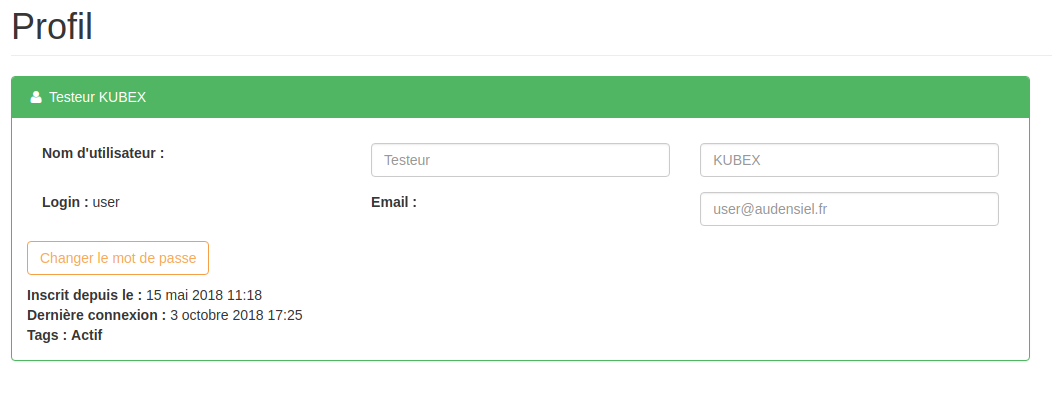
\includegraphics[width=\textwidth]{images/profil.png}
	\caption{\label{fig:profil} Profil utilisateur}
\end{figure}


%\subsection{Paramètres utilisateurs}
%\label{subsec:paramètres}

% Cette partie est pour le moment vide tout comme la template. Elle est destinée à accueillir les préférences utilisateurs (messages,emails, permissions, notifications,automatismes...) une fois que toutes ces dernières auront été implémentées. Cette page servira alors d'interface vers une modèle de configuration utilisateur et ses APIs, et la documentation devra être complétée en conséquence.

\subsection{Recherche}
\label{subsec:search}

Au contraire des autres fonctionnalités, l'accès à cette page ne se fait pas au moyen d'un bouton de menu, mais avec la barre de recherche globale située en haut du menu latéral.

\begin{figure}[h!]
	\centering
	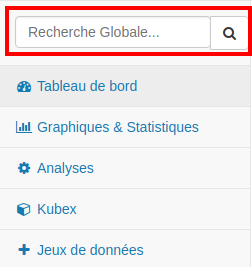
\includegraphics[width=0.5\textwidth]{images/globalSearch.png}
	\caption{\label{fig:globalSearch} Recherche dans l'ensemble des données}
\end{figure}

Cette fonction va rechercher dans les jeux de données, analyses, et messages toutes les entrées contenant les mots indiqués, que ce soit en tant que mot-clés, dans le titre, la description, ou l'utilisateur. Cette fonction est destinée à regrouper avec une seule recherche toutes les ressources disponibles sur un sujet, afin d'obtenir une vue d'ensemble d'une simple clic.


\section{Administration}
\label{sec:admin}

L'interface d'administration permet aux administrateurs d'Audensiel de gérer les utilisateurs, les différents \emph{Kube}, et de répondre rapidement aux tickets ouverts. L'accès à la page en elle-même est réservé aux utilisateurs disposant de droits d'administration sur le site.

\begin{figure}[h!]
	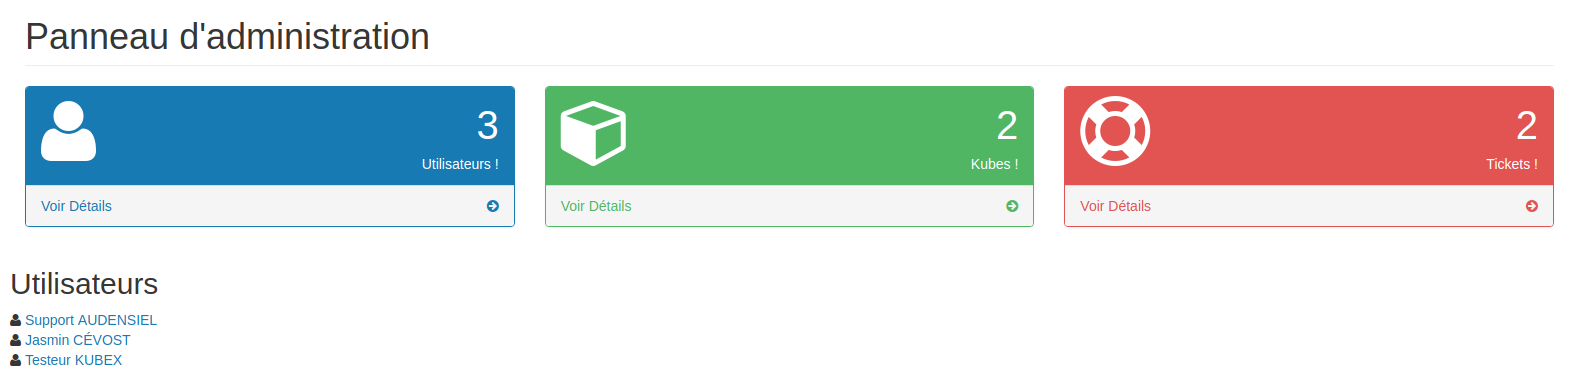
\includegraphics[width=\textwidth]{images/pageAdmin.png}
	\caption{\label{fig:admin} Interface d'administration}
\end{figure}

Cette interface propose l'accès aux trois catégories détaillées ci-dessus :

\begin{description}
	\item[Utilisateurs] Donne un accès administrateur à tous les profils d'utilisateur pour modifier leurs droits et éventuellement mot de passe (en cas de perte)
	\item[Kubex] Donne un accès administrateur à tous les Kubex pour accéder et gérer leur configuration à distance
	\item[Tickets] Liste les tickets en cours pour permettre de se les assigner et résoudre les demandes utilisateurs.
\end{description}

Depuis cette interface, les administrateurs Audensiel pourront donc directement effectuer des tâches d'administration sur les éléments de ces trois catégories, leur permettant un accès rapide, intuitif et réduisant le temps nécessaire à leurs interventions.

\chapter{Documentation du code}

Ce projet contient tous les fichiers nécessaires au déploiement d'une interface utilisateur pour le cloud Kubex, y compris une base de données basique et les prérequis de l'environnement virtuel.

\section{Lancement du serveur}

\subsection{Initialisation}


Installer et configurer postgreSQL si nécessaire.

\begin{verbatim}
sudo apt-get install postgresql postgresql-contrib
sudo -su postgres
psql
postgres=> CREATE USER audensiel PASSWORD 'Audensiel2018';
postgres=> CREATE DATABASE kubex;
\end{verbatim}

Charger la base de données kubex :

\begin{verbatim}
psql -U audensiel kubex < backup/database.psql
\end{verbatim}

Pour sauvegarder les modifications de la base de données dans le fichier \emph{backup.psql}, la commande est :

\begin{verbatim}pg_dump -a kubex -f backup/database.psql\end{verbatim}

Ensuite, installer les modules nécessaires dans un environnement Python V3.5 :

\begin{verbatim}
pip install -r cloud_GUI/requirements.txt
\end{verbatim}

Une fois l'environnement initialisé, vérifier que la base de données est à jour avec les modèles django et réaliser les migrations si besoin. Ceci permet également de tester le bon fonctionnement ainsi que la configuration de l'environnement et de la base de données.

\begin{verbatim}
python manage.py makemigrations
python manage.py migrate
\end{verbatim}



\subsection{Démarrage rapide}
\label{subsec:quickstart}

\paragraph{Script de lancement global}~\\
Pour plus de simplicité, les commandes lançant le serveur Django, le serveur de calcul Celery, et le serveur de réception des données Bottle sont rassemblées dans le fichier \emph{launcher.sh} qu'il suffit d'appeler en ligne de commandes :

\begin{verbatim}
./launcher.sh
\end{verbatim}


Les outputs de chacun de ces scripts seront stockés dans le répertoire \emph{logs}, avec pour chaque processus la sortie standard dans un fichier \emph{.out} et la sortie d'erreur dans un \emph{.err}, de la façon suivante :

\begin{itemize}
	\item serveur : GUI.*
\end{itemize}

\paragraph{Détail des commandes}~\\

Les différentes commandes qui le composent peuvent être lancées séparément, à commencer par l'activation de l'environnement virtuel :

\begin{verbatim}
source my_env/bin/activate
\end{verbatim}

L'environnement virtuel permet de conserver des versions fonctionnelles pour tous les modules Python, et également de pouvoir être déployé rapidement sur une nouvelle infrastructure.

Pour sortir de cet environnement virtuel, il suffira de taper : \begin{verbatim}deactivate\end{verbatim}.

Enfin, lancer localement le serveur de développement

\begin{verbatim}
python manage.py runserver 0:8080
\end{verbatim}

Pour y accéder ensuite, entrer l'adresse \href{http://localhost:8080}{http://localhost:8080} (ou remplacer \emph{localhost} par l'adresse IP du serveur depuis un PC distant).\\


Les comptes réservés permettant d'accéder à cette interface dont :

\begin{description}
	\item[audensiel (mdp:Audensiel2018)] Compte administrateur
	\item[user (mdp:user123)] Compte de test standard
\end{description}





\section{Langages et environnement}

Le code de la partie serveur est constitué des langages HTML, CSS et Javascript pour la partie front-end, tandis que la partie back-end est assurée par le framework django REST dans un environnement virtuel en python v3.5. Les modules requis pour cet environnement peuvent être importés depuis le fichier \emph{requirements.txt} du dossier \emph{backup}.\\

La base de donnée utilisée est postgreSQL; une copie de sauvegarde de la base de donnée utilisée pour le développement se trouve dans le fichier \emph{database.psql}. Le déploiement en production est prévu via un serveur apache2 qui sera configuré ultérieurement.


\section{Back-end : Django REST}
Le back-end de l'interface graphique est assuré par le framework Django  en utilisant un environnement virtuel de Python v3.5, dont les librairies sont installables par \emph{pip} en utilisant le fichier versionné \emph{requirements.txt}. La base de données postgreSQL dont le backup se situe dans le fichier \emph{backup.psql} doit également être opérationnelle.\\


\subsection{Structure des dossiers}
L'organisation des dossiers de l'interface du cloud s'effectue sur la base du Django REST Framework : dans le dossier principal se trouvent le dossier racine (\emph{Kubex\_GUI}), ainsi que le dossier de l'application (\emph{data}). Viennent s'y ajouter les dossier servant à stocker des données, logs, d'autres modules ou scripts.\\

L'architecture générale est présentée ci-dessous, les fichiers permettant de lancer et configurer le serveur ont été soulignés.

\begin{description}
	
	
	\item[backup/] dossier contenant les données de sauvegarde comme \emph{requirements.txt}, \emph{database.psql} et une copie des configurations des 
	\item[data/]** Application web principale contenant l'essentiel du code et templates
	\item[doc/] Documentation du GUI, incluant le manuel utilisateur
	\item[kubex\_data/]* Stockage local des jeux de données et configurations
	\begin{description}
		\item[datasets/] Jeux de données classés par numéro de Kubex
		\item[config/] Fichiers de configuration des Kubes et senseurs
	\end{description}
	\item[Kubex\_GUI/] Dossier principal contenant les fichiers de configuration de django
	\begin{description}
		\item[settings.py] \underline{Configuration générale du serveur}
		\item[static/] Fichiers statiques du serveur (JavaScript, CSS, images...)
	\end{description}
	\item[launcher.sh] \underline{Script de lancement global de tous les services}
	\item[logs/]* Contient les logs de tous les modules
	\item[manage.py] \underline{Script principal lançant le serveur web}
	\item[scripts/]* Lien (symbolique) vers les scripts d'analyse\ref{subsec:scripts}
	\item[tmp/]* Dossier de stockage temporaire des données en provenance des BoS
\end{description}
~\\
* Le contenu de ces dossiers n'est pas pris en compte par \emph{git}.\\
** L'essentiel des fonctions du serveur web se trouvant dans le dossier \emph{data}, la liste détaillée est présentée ci-dessous pour plus de clarté :
 
\begin{description}
\item[admin.py]* Fonctionnalités réservées aux administrateurs
\item[apis.py] Fonctions d'interaction utilisateur/serveur (API)\ref{subsec:API}
\item[apps.py]* Configuration de l'application (data)
\item[celery.py]* Configuration de Celery
\item[migrations/] Migrations effectuées et en cours (par ex: modèles dans DB)
\item[models.py] Modèles de données\ref{subsec:model}
\item[serializers.py]* Sérialiseurs associés aux modèles
\item[tasks.py] Tâches exécutables par Celery\ref{subsec:task}
\item[templates/] Templates html utilisées pour l'affichage des pages\ref{subsec:template}
\begin{description}
	\item[panel/] Sous-templates d'éléments intégrés aux pages
\end{description}
\item[templates-factory/] Modèles de templates pour le développement futur
\item[tests.py]* Tests et validation
\item[urls.py] Mapping des urls vers les pages\ref{subsec:url} (\emph{views.py}) ou APIs (\emph{apis.py})
\item[views.py] Génération dynamique des pages\ref{subsec:view}
\end{description}
 
* Pour ces fichiers, seule la configuration de base est utilisée
 
\subsection{Navigation sur le site}
\label{subsec:url}
La navigation entre les différentes pages de l'interface se fait d'après le mapping réalisé dans le fichier \emph{urls.py}. Ces URLs correspondent en général à deux types de fonctionnalités : des \emph{API} permettant d'interagir avec le serveur au moyen de fonctions du module \emph{apis.py} (URLs commençant par \emph{api/<model>/})\ref{subsec:API} , ou bien des \emph{vues} basées sur des fonctions du module \emph{views.py} générant dynamiquement des pages HTML\ref{subsec:view}.

\begin{table}[!h]
\begin{tabular}{|c|c|c|}
\hline
URL & Fonction & Description \\
\hline
/ & views.root & Redirige vers 'dashboard' \\
index & views.index & Redirige vers 'dashboard' \\
login & auth\_views.LoginView.as\_view & Page de connexion \\
admin & views.admin & Page d'administration \\
dashboard & views.dashboard & Tableau de bord \\
graphics & views.graphics & Page de visualisation graphique \\
analysis & views.analysis & Page d'analyse \\
api/analysis/launch &  apis.launchAnalysis.as\_view & Lancement d'une analyse \\
kubex & views.kubex & Page des Kubex \\
api/kubex/status & apis.getKubexConfig.as\_view & Informations sur le Kube \\
api/kubex/config & apis.setKubexConfig.as\_view & Modification du Kube \\
datasets & views.datasets & Jeux de données \\
inbox & views.inbox & Boîte de messagerie \\
api/algorithm/<id> & apis.getAlgorithmParameters.as\_view & Chargement d'un algorithme \\
api/algorithm/list/ & apis.getAlgorithms.as\_view & Liste les algorithmes \\
tasks & views.tasks & Page listant les analyses \\
alerts & views.alerts & Notifications \\
api/alerts/delete/<id> & apis.deleteAlert.as\_view & Supprimer une notification \\
profile & views.profile & Profil utilisateur \\
settings & views.settings & Paramètres (TODO) \\
logout & auth\_views.LogoutView.as\_view & Déconnexion \\
search & apis.searchQuery.as\_view & Lancement d'une recherche \\
support & views.support & Centre de support/tickets \\
support/add & apis.addTicket.as\_view & Création d'un ticket \\
manual & apis.getManual.as\_view & Affiche le manuel utilisateur \\
api/dataset/list/ & apis.getDatasetList.as\_view & Liste les jeux de données (par format) \\
api/dataset/add & apis.addDataset.as\_view & Ajout d'un jeu de données \\
api/dataset/edit & apis.editDataset.as\_view & Edition des métadonnées \\
api/dataset/<id> & apis.getDatasetMetadata.as\_view & Chargement des métadonnées \\
api/dataset/delete/<id> &  apis.deleteDataset.as\_view & Suppression d'un jeu de données \\
api/dataset/column &  apis.getDatasetColumns.as\_view & Chargement des données \\
api/dataset/search &  apis.searchDataset.as\_view & Recherche d'un Dataset \\
api/message/add & apis.addMessage.as\_view & Ecriture d'un message \\
\hline
\end{tabular}
\caption{\label{tab:urls} Correspondances des URLs}
\end{table}

\subsection{Génération des pages}
\label{subsec:view}

Chacune des pages parcourues par l'utilisateur est générée dynamiquement par une fonction contenue dans le module \emph{views.py}. Ces fonctions génèrent les pages en se basant sur trois éléments distincts : la requête envoyée par l'utilisateur, la template de la page à renvoyer, et enfin le contexte qui permettra de modifier dynamiquement la template.

Après avoir vérifié l'authentification de l'utilisateur, la fonction appelée via \emph{urls.py} charge la template appropriée, puis le contexte général (dictionnaire) utilisé pour les barres de menus (via la fonction \emph{baseView}), et enfin ajoute les éléments de contexte spécifiques à chaque page dans le dictionnaire.
Elle utilise ensuite la fonction \emph{HttpResponse} afin de renvoyer le \emph{render} de la template en utilisant les informations présentes dans la requête et le contexte.

\subsection{Contenu des pages}
\label{subsec:template}

Le contenu de chaque page est défini dans le dossier \emph{templates}; celles ci correspondent généralement à une page qui sera générée par une fonction de \emph{views.py}, avec deux exceptions notables :
\begin{itemize}
	\item La template \emph{base.html} sert de base pour toutes les autres. Elle en définit la forme général, le menu, ainsi que les scripts JavaScript généraux. Les templates qui en héritent insèreront simplement leur(s) code(s) spécifique(s) aux endroits appropriés.
	\item Les sous-templates du sous-dossier \emph{panels} correspondent à des éléments répétés dans plusieurs pages, correspondant à la représentation d'instances des modèles
\end{itemize}

Dans une page classique (ici \emph{datasets.html}), on peut retrouver les éléments dynamiques suivants :

\begin{verbatim}

\end{verbatim}

Cette balise signifie que la template hérite de celle comprenant la forme générale et les menus. Lors du rendu, la page web finale inclura le code de la template ciblée à l'intérieur de \emph{base.html}, et le positionnera selon les balises suivantes :

\begin{verbatim}

<liens CSS>


<code de la template>


<liens JavaScript>

\end{verbatim}

Ces "blocs" délimités par les balises \emph{\{\%block <nom>\%\}} et \emph{\{\% endblock \%}\} définissent les segments qui seront inclus dans la template \emph{base.html}.Tout le code présent à l'intérieur d'un bloc sera inséré entre les balises correspondantes de la template \emph{base.html}.\\

Le processus inverse est également possible : il consiste à inclure (au moyen de l'instruction \emph{include})des segments de code HTML + Django préformatés à l'intérieur d'une page. Cette méthode possède deux avantages principaux : elle permet de réutiliser un template simple dans l'ensemble des pages tout en conservant une unique copie modifiable, et ils permettent également de redéfinir le contexte particulier pour ce sous-template.\\

L'exemple ci-dessous illustre la façon dont les panneaux correspondant à l'ensemble des datasets sont générés de façon simple et efficace :

\begin{verbatim}



\end{verbatim}

\begin{itemize}
	\item La boucle \emph{for} permet de générer le code pour chaque instance de \emph{datasets}
	\item L'instruction \emph{include} indique de charger l'ensemble de la sous-template \emph{panels/dataset.html} à cet emplacement, et restreint le contexte uniquement au \emph{dataset} actuellement examiné par la boucle
	\item Le \emph{render} générera à chaque itération le panneau d'information correspondant au jeu de données au moyen du contexte fourni
\end{itemize}
~\\
Une autre fonctionnalité utile offerte par Django pour les templates est de générer automatiquement les liens vers les fichiers statiques. Pour ce faire, le ou les emplacements des fichiers statiques doivent être définis dans \emph{settings.py} (correspondant ici au dossier \emph{Kubex\_GUI/static}). L'instruction \emph{\{\% load static \%\}} cherchera alors les fichiers demandés parmi les fichiers statiques pour générer les liens dynamiquement, même en cas de déplacement des fichiers.

\begin{verbatim}

<link href="" rel="stylesheet">
<link href="" rel="stylesheet">
<script src=""></script>
<script src=""></script>
\end{verbatim}

Pour finir, il est également possible de fournir une sécurité contre les attaques de type \emph{Cross Site Request Forgery} au moyen d'un jeton généré lors de l'authentification et reporté dans chaque formulaire, via l'instruction suivante :

\begin{verbatim}

\end{verbatim}

Cette instruction génère un jeton d'authentification propre à la session en cours, qui devra être identique dans toutes les requêtes effectuées par l'utilisateur, et évitera ainsi d'effectuer des actions non désirées en cliquant sur un lien non généré par le site.

\subsection{Modèles de données}
\label{subsec:model}
Les données gérées par l'interface graphiques sont stockées dans une base de données postgreSQL dont django gère les modèles. Les sections ci-dessous présentent les modèles exprimés dans le module \emph{models.py} qui correspondent ensuite à des tables dans la base de données postgreSQL dont le nom sera \emph{data\_<modèle>}. Django est en charge de la gestion des contraintes, liens entre les tables et clés primaires. Lorsque ce n'est pas explicitement précisé autrement, la clé primaire de chaque modèle est un champ entier \emph{id} auto-incrémental.\\

Les relations de type \emph{ManyToMany} impliquent la création d'une table intermédiaire (\emph{data\_<modèle1>\_<modèle2>}) qui servira de lien entre deux modèles.
Les relations de type \emph{GenericForeignKey} référencent une autre entrée pouvant appartenir à différents modèles. Dans ce but, les champs \emph{object\_id} et \emph{content\_type\_id} seront créés pour référencer le type de modèle au sein de la table \emph{django\_content\_type} (\emph{content\_type\_id}), et l'identifiant au sein de la table associée à ce modèle (\emph{object\_id}). Une \emph{GenericRelation} est également créée dans les modèles ciblés afin de permettre les requêtes dans le sens inverse.

\subsubsection{Kubex}
\begin{tabular}{|l|c|c|}
	\hline
	\textbf{Nom} & \textbf{Type} & \textbf{Description} \\
	\hline
	IP & GenericIPAddressField & Adresse IP du \emph{Kube} \\
	SN & PositiveIntegerField & Numéro de série du \emph{Kube}* \\
	name & CharField & nom du \emph{Kube} \\
	owner & ForeignKey('KubexUser') & Administrateur du \emph{Kube} \\
	users & ManyToManyField('KubexUser') & Utilisateurs de ce \emph{Kube} \\
	\hline
\end{tabular}
~\\
*Ce champ contitue la clé primaire du modèle.\\\\
Les données sont triées dans l'ordre du champ \emph{name}.

\subsubsection{Sensor}
\begin{tabular}{|l|c|c|}
	\hline
	\textbf{Nom} & \textbf{Type} & \textbf{Description} \\
	\hline
	Kubex & ForeignKey & Kubex d'appartenance \\
	SID & PositiveInteger Field & ID du capteur \\
	config & FileField & Fichier de configuration \\
	title & CharField & Nom du capteur \\
	data & GenericRelation & Lien avec les Datasets \\
	\hline
\end{tabular}

\subsubsection{Message}
\begin{tabular}{|l|c|c|c|}
	\hline
	\textbf{Nom} & \textbf{Type} & \textbf{Description} & \textbf{Défaut}\\
	\hline
	sender & ForeignKey('auth.User') & Expéditeur & request.user \\
	recipient & ForeignKey('auth.User') & Destinataire & \\
	title & CharField & Objet du message & \\
	time & DateTimeField & Date d'envoi & auto\_add\_now \\
	description & CharField & Contenu du message & \\
	status & CharField & Non Lu/Lu/Archivé & Non Lu\\
	\hline
\end{tabular}
~\\~\\
Les données sont triées dans l'ordre inverse du champ \emph{time}.

\subsubsection{Ticket}
\begin{adjustbox}{center}\begin{tabular}{|l|c|c|c|}
		\hline
		\textbf{Nom} & \textbf{Type} & \textbf{Description} & \textbf{Défaut}\\
		\hline
		owner & ForeignKey('auth.User') & Auteur du ticket & request.user \\
		in\_charge & ForeignKey('auth.User') & Admin en charge & audensiel \\
		creation\_time  & DateTimeField & Création  du ticket & auto\_add\_now \\
		modification\_time & DateTimeField & Dernière mise à jour du ticket & auto\_now \\
		title & CharField & Titre du ticket & \\
		status & CharField & Nouveau/Assigné/Résolu/En attente & Nouveau \\
		description & CharField & Description du problème/demande & \\
		keywords & ManyToManyField('Keyword') & Tags associés & \\
		\hline
\end{tabular}\end{adjustbox}
~\\
Les données sont triées dans l'ordre inverse du champ \emph{modification\_time}.

\subsubsection{Dataset}
\begin{adjustbox}{center}\begin{tabular}{|l|c|c|c|}
		\hline
		\textbf{Nom} & \textbf{Type} & \textbf{Description} & \textbf{Défaut}\\
		\hline
		kubex & ForeignKey('Kubex') & Kubex d'origine & \\
		description & CharField & Description du jeu de données & \\
		title & CharField & Titre du jeu de données & \\
		data\_format  & CharField & Table/Image/Audio/Vidéo & Table \\
		creation\_time & DateTimeField & Création & auto\_now\_add \\
		modification\_time & DateTimeField & Dernière modification & auto\_now \\
		keywords & ManyToManyField('Keyword') & Mots-clés associés & \\
		data & FileField & Fichier de données & \\
		origin & GenericForeignKey & Origin du Dataset & \\
		\hline
\end{tabular}\end{adjustbox}
~\\
Les données sont triées dans l'ordre inverse du champ \emph{modification\_time}.

\subsubsection{Alert}
\begin{adjustbox}{center}\begin{tabular}{|l|c|c|c|}
		\hline
		\textbf{Nom} & \textbf{Type} & \textbf{Description} & \textbf{Défaut}\\
		\hline
		owners & ManyToManyField('auth.User') & Liste de diffusion & \\
		status & CharField & Indication/Erreur/Validation/Avertissement & Indication \\
		time  & DateTimeField & Date de la notification & auto\_now\_add \\
		title & CharField & Titre de la notification & \\
		source & GenericForeignKey & Source de la notification & \\    
		\hline
\end{tabular}\end{adjustbox}

~\\
Les données sont triées dans l'ordre inverse du champ \emph{time}.

\subsubsection{Analyse}
\begin{adjustbox}{center}\begin{tabular}{|l|c|c|c|}
		\hline
		\textbf{Nom} & \textbf{Type} & \textbf{Description} & \textbf{Défaut}\\
		\hline
		status & CharField & en cours/arrêtée/en erreur/terminée & en erreur \\
		owner & ForeignKey('auth.User') & Propriétaire de l'analyse & request.user \\
		kubex & ForeignKey('Kubex') & Kubex associé & \\
		datasets & ManyToManyField('Dataset') & Datasets d'enteée & \\
		creation\_time & DateTimeField & Date de lancement & auto\_now\_add \\
		modification\_time & DateTimeField & Dernier accès & auto\_now \\
		title & CharField & Titre de l'analyse & \\
		description & CharField & Description de l'analyse & \\
		algorithm & ForeignKey('Algorithm') & Algorithme utilisé & \\
		progress  & DecimalField & avancement de l'nalyse (\%) & 0\% \\
		inputs & JSONField & Données d'entrée & \\
		parameters & JSONField & Paramètres utilisés & \\
		command & Charfield & Commande de lancement & \\
		results & GenericRelation('Dataset') & permet le lien avec le dataset généré & \\
		\hline
\end{tabular}\end{adjustbox}

~\\
Les données sont triées dans l'ordre inverse du champ \emph{modification\_time}.

\subsubsection{Algorithm}
\begin{adjustbox}{center}\begin{tabular}{|l|c|c|c|}
		\hline
		\textbf{Nom} & \textbf{Type} & \textbf{Description} & \textbf{Défaut}\\
		\hline
		algo\_type  & CharField & \begin{minipage}{6cm}\centering Régression/Classification/\\Statistiques/Apprentissage/Analyse\\ factorielle/Traitement d'image\end{minipage} & \\
		data\_format & CharField & Table/Image/Audio/Vidéo & Table \\
		title & CharField & Titre de l'algorithme & \\
		inputs & JSONField & Données d'entrée &  \\
		parameters & JSONField & Paramètres & \\
		description & CharField & Description de l'algorithme & \\
		command & CharField & Commande de lancement & \\
		progression\_regex & Charfield & Format de l'indicateur de progression &  \\
		output & JSONField & Données de sortie & \\
		\hline
\end{tabular}\end{adjustbox}
~\\
Les données sont triées dans l'ordre du champ \emph{title}.

\subsubsection{Keyword}
\begin{tabular}{|l|c|c|c|}
	\hline
	\textbf{Nom} & \textbf{Type} & \textbf{Description} & \textbf{Défaut}\\
	\hline
	word & CharField & mot-clé & NA \\
	\hline
\end{tabular}
~\\~\\
Les données sont triées dans l'ordre du champ \emph{word}

\subsection{APIs}
\label{subsec:API}
Une majorité des fonctions offertes par Django réside dans les \emph{APIs} grâce auxquelles l'utilisateur peut interagir avec les données. Ces APIs sont rassemblées dans le fichier \emph{apis.py} et sont généralement appelées via une fonction JavaScript\ref{sec:javascript} renvoyant à une adresse de la forme \emph{api/<modèle>/<fonction>}.\\

Elles sont constituées d'une classe dérive de \emph{APIView}, dont au moins une fonction est nommée \emph{get} ou \emph{post} et correspond à la méthodes HTML associée. Lors de l'envoi d'une requête à une de ces fonctions, l'objet \emph{request} contiendra toutes les données associées, principalement l'utilisateur dans \emph{request.user}, et les données dans \emph{request.query\_params} pour un GET ou \emph{request.data} pour un POST.\\

Les APIs vont alors vérifier que l'utilisateur est authentifier, charger les modèles requis par la requête, éventuellement procéder à des traitements supplémentaires puis renvoyer une réponse HTML. Cette réponse sera généralement sous un format JSON accompagnée du code HTML indiquant le succès ou l'échec de la requête.

\subsubsection{Manual}
On accède à cette API en cliquant sur les liens \emph{Manuel} proposés sur la page d'authentification et le menu supérieur\ref{subsec:manual}, qui redirigent vers l'URL \emph{/manual}.\\

Cette URL redirige vers la classe \emph{getManual} dont la méthode \emph{get} récupère simplement le fichier \emph{doc/user-manual.pdf} et l'affiche dans la fenêtre actuelle. Ce document contient la documentation utilisateur de la GUI qui peut être trouvée au chapitre\ref{chap:manual}, à l'exception de la section réservée aux administrateurs\ref{sec:admin}.

\subsubsection{Search}
On accède à cette API par le champ \emph{recherche globale} situé dans le menu latéral gauche\ref{subsec:search}, qui renvoie à l'url \emph{/search?content=<kw1,kw2...>}.
La fonction \emph{get} de la classe \emph{searchQuery} effectue alors une recherche dans les jeux de données, analyses, et messages (à ce jour par mots exacts, insensibles à la casse) et renvoie une liste de résultats dans la page \emph{search}\ref{subsec:search}.\\

Cette API génère une page de la même façon que les fonctions du module \emph{views.py}\ref{subsec:view}, à la différence qu'elles prennent en entrée une requête complète, puis effectuent 3 recherches poussées dans la base de données au moyen de fonctions \emph{Q} servant à combiner les critères, et de \emph{iregex} permettant de chercher une expression régulière de façon insensible à la casse. Chacune des requêtes chargent un élément du contexte (\emph{query\_<modèle>} avec <modèle> parmi dataset, analyse, ou message)

\subsubsection{Algorithmes}
On accède à ces API dans la page \emph{analyse}\ref{sec:analyses}, lors de la sélection de l'algorithme utilisé pour l'analyse.Elles permettent à l'utilisateur de sélectionner et paramétrer un algorithme d'analyse pour répondre de la façon la plus adaptée possible à ses besoins.

\paragraph{Liste des algorithmes}
En sélectionnant le format des données, un appel à l'URL \emph{/api/algorithm/list?dataFormat=<T|A|I|V>} redirigeant vers la méthode \emph{get} de la classe \emph{getAlgorithms} va permettre de récupérer la liste des algorithmes applicables.
La liste (titre et identifiant) des algorithmes correspondant au format de données choisi (\emph{dataFormat} valant T/A/I/V pour Table/Audio/Image/Vidéo) sera renvoyée au format JSON pour être affichée dans le champ adéquat par un JavaScript, accompagné du code 200. En cas d'erreur, un code 500 et un message d'erreur seront retournés.

\paragraph{Chargement d'un algorithme} Lorsque l'on sélectionne un algorithme parmi la liste proposée dans le menu déroulant, un appel à l'URL \emph{/api/algorithm/(?P<algo\_id>\d+)} redirigeant vers la méthode \emph{get} de la classe \emph{getAlgorithmParameters} permettra de charger les différents champs requis pour les données d'entrée et les paramètres qui seront utilisés lors de l'analyse. La valeur de \emph{<algo\_id>} est utilisée pour effectuer la requête de l'algorithme dans la base de données, l'API renvoie toutes ses propriétés sous forme de JSON ainsi qu'un code HTML 200 en cas de succès, un message d'erreur et un code HTML 500 en cas d'erreur.\\
Ces propriétés serviront à générer automatiquement tous les champs requis au paramétrage de l'algorithme\ref{subsec:analyse_js}.

\subsubsection{APIs des analyses}
Une fois tous les champs requis requis, l'utilisateur peut lancer une analyse, ce qui se traduira par un appel à l'url \emph{api/analysis/launch}, qui transmettra toutes les informations fournies à la à la fonction \emph{post} de la classe \emph{launchAnalysis}. Celle-ci est en charge de créer l'objet \emph{Analyse} associé et de le transmettre à la tâche Celery \emph{launchAnalysis}\ref{subsec:task}.\\

Elle crée également l'objet \emph{PeriodicTask} associé à cette Analyse si celui-ci est requis, ce qui permet de lancer cette même analyse à des intervalles réguliers sur les nouvelles données générées par les mêmes capteurs.\\

En cas de succès de la transmission de l'analyse à Celery, une confirmation portant le code HTTP 201 est renvoyée. En cas d'échec, un message d'erreur accompagné du code HTTP 500 est renvoyé. Lors de l'ajout d'une tâche périodique, son succès ou son erreur sont précisés dans le message de confirmation de l'analyse mais en changent pas le code de confirmation de l'analyse en elle-même. De plus, cette première confirmation signifie simplement que la requête a pu être interprétée et transmise à Celery, le succès ou l'échec de la tâche Celery sera quant à lui transmis par le biais de notifications.

\subsubsection{APIS des jeux de données}

\paragraph{getDatasetMetadata} 
Cette fonction permet de récupérer les informations relatives à un dataset, comme son titre, description, et champs. cette fonction est appelée depuis une requête GET à l'adresse \emph{/api/dataset/(?P<data\_id>\d+)} et renvoie un format JSON contenant les informations demandées sur le dataset d'identifiant \emph{<data\_id>}.

\paragraph{addDataset} 
Cette fonction permet d'ajouter un nouveau dataset aux données d'un senseur existant. En envoyant une requête POST du formulaire présent dans l'onglet \emph{Jeux de données} à l'URL \emph{/api/dataset/add}, l'API va télécharger le fichier et créer l'entrée correspondant au Dataset dans la base de données. La confirmation se fera par l'envoi d'un statut HTTP 201.


\paragraph{getDatasetColumns}
Cette fonction permet de renvoyer les données contenues dans les colonnes d'un dataset. Elle est utilisée exclusivement depuis l'interface \emph{Visualisation graphique} au moyen d'un appel  l'URL \emph{/api/dataset/column} où une requête POST détaille les colonnes de données requises par l'utilisateur. Cette API va alors renvoyer un JSON de format similaire où les valeurs de chaque colonne auront été ajoutées. Ceci permettra aux fonctions d'affichage  Javascript de générer les courbes, images ou autres visualisations demandées par l'utilisateur.

\paragraph{editDataset} Cette API permet d'éditer directement un Dataset depuis l'onglet associé. Une fois le formulaire correspondant au Dataset validé, un appel POST à l'URL \emph{api/dataset/edit} va mettre à jour les informations du Dataset de la base de données (les fichiers eux-mêmes ne sont pas directement modifiables), et renverra un message de confirmation accompagné du code HTTP 200 en cas de succès.

\paragraph{deleteDataset} La suppression d'un dataset est possible au moyen de cette API, passant par un appel à une requête DELETE adressée à l'URL \emph{api/dataset/delete/<id>}. Une fois l'authenticité de l'utilisateur et ses droits sur le dataset validés, le dataset sera supprimé de la base de données et son fichier supprimé. Une amélioration possible permettant d'aviter les erreurs même après confirmation pourrait être de déplacer temorairement ce dataset vers un dossier de \emph{backup} où il pourra être récupéré.

\paragraph{getDatasetList}
Cette fonction permet d'obtenir la liste des Datasets d'un format choisi, afin de permettre au front-end de générer une liste des datasets pouvant être sélectionnés par l'uilisateur, ce ce soit pour une visualisation ou une analyse. Pour appeler cette focntion, une requête GET est transmise à l'URL \emph{/api/dataset/list?dataFormat=<T|V|I|A>}, où la lettre T,V,I ou A spécifie le format de Table, Audio, Vidéo ou Image. La liste des datasets est alors renvoyée au format JSON sous forme d'un tableau de doublets identifiant/titre pour permettre leur sélection.

\paragraph{searchDataset} Cette API permet d'effectuer une recherche au sein des Datasets à disposition de l'utilisateur. Elle est accessible depuis la barre de recherche des datasets, au moyen d'une requête POST envoyée à l'adresse \emph{/api/dataset/search?content=<kw1,kw2...>}. L'API va chercher les mots fournis dans \emph{<kw1,kw2>} dans le titre, la description et les mots-clés des datasets et retourner la liste des identifiants des datasets correspondants. Pour les mots clés, une correspondance exacte sera utilisée, cependant la recherche dans le titre et la description seront insensibles à la casse.

\subsubsection{APIs des tickets}
Depuis la page \emph{tickets}, en validant le formulaire proposé postant les données à l'URL \emph{/api/ticket/add}, la class \emph{addTicket} ajoute un nouveau ticket. Un code HTML 201 est renvoyé pour signifier le succès de cette tâche; les administrateurs recevront dès lors une notification permettant d'assigner et résoudre ce ticket.




\section{Front-end : JavaScript}
\label{sec:javascript}

Les fichiers javascript permettent de lancer les fonctionnalités dans le front-end et faire la communication entre le front-end et le serveur, assurer le bon fonctionnement du GUI. Pour l'instant, il y a 6 fichiers javascript personnalisés: \emph{base.js}, \emph{page\_analysis.js}, \emph{page\_dashboard.js}, \emph{page\_dataset.js}, \emph{page\_graphics.js} et \emph{page\_kubex.js}, qui fournissent les fonctions pour les templates \emph{base.html}, \emph{analysis.html}, \emph{dashboard.html}, \emph{datasets.html}, \emph{graphics.html} et \emph{kubex.html}. 

\subsection{base.js}

\paragraph{Dépendances} : jquery.min.js, bootstrap.min.js, bootstrap-tagsinput.min.js, typeahead.bundle.min.js.

\paragraph{Variables globales}~\\
Ce fichier ne présente aucune variable globale.

\paragraph{Fonctions}~\\
\begin{description}
	\item[function substringMatcher]: Reçoit un input de type "string", renvoie une fonction de détection utilisée par librairie \emph{typeaheadjs} pour détecter l'input string, après afficher les résultats dans l'élément html \emph{input\#search-input}.
	
	\item[function handleSearch]: Obtient les contenus de barre de recherche à gauche de la page, puis redirige à la page \emph{search} avec ces contenus comme paramètre de recherche. S'il n'y a pas contenu dans barre de recherche cette fonction va passer "null" comme paramètre.
	
	\item[function responseMsg]: Une fonction globale utilisé pour renvoyer une notification dans front-end quand javascript reçoit la réponse du serveur.
	
	\item[function confirmation]: Une fonction globale utilisé pour afficher un bloc de confirmation dans le front-end quand l'utilisateur essaie de supprimer un dataset depuis la page "Tableau de Bord" ou "Jeux de données".
	
	\item[function deleteDataset]: Une fonction globale utilisé pour supprimer un dataset dans la page "Tableau de Bord" ou "Jeux de données", qui va envoyer une requête DELETE à l'api \emph{deleteDataset} du serveur (url: \emph{api/dataset/delete/(?P<data\_id>\\d+)}), et une fois supprimé recharge de la page.
	
	\item[function deleteDataset]: Une fonction globale utilisé pour supprimer une notification dans page "Notifications", qui va envoyer une requête DELETE à l'api \emph{deleteAlert} du serveur (url: \emph{api/alerts/delete/(?P<alert\_id>\\d+)}).
\end{description}

\subsection{page\_analysis.js}
\paragraph{Dépendances} : jquery.min.js, bootstrap.min.js, bootstrap-multiselect.js, js.cookie.js.

\paragraph{Variables globales}~\\
\begin{description}
	\item[datasets] enregistrement des datasets renvoyés par le serveur
	\item [input\_infos] enregistrement de l'input d'algorithme renvoyé par le serveur
	\item [params\_infos] enregistrement du paramètre d'algorithme renvoyer par le serveur
	\item [PERIOD\_UNIT] enregistrement des valeurs nécessaires pour créer les champs de \emph{periodic\_task}
\end{description}

\paragraph{Fonctions}~\\
\begin{description}
	\item[function setDatasetFormat]: Une fonction qui contrôle l'affichage et cache du bloc \emph{algoType\_container} et bloc \emph{selectBox\_container} selon la sélection du type de donnée par l'utilisateur.
	
	\item[function getDatasetList]: Une fonction qui fait un appel GET à l'api \emph{getDatasetList} du seveur (url: \emph{api/dataset/list}), passe le format de dataset comme paramètre et obtient une liste de datasets correspondant, incluant le titre et l'id du dataset.
	
	\item[function getData]: Une fonction qui fait un appel GET à l'api \emph{getDatasetMetadata} du seveur (url: \emph{api/dataset/(?P<data\_id>\\d+)}), passe l'id de un dataset comme paramètre et obtient l'info du dataset correspondant, incluant le titre, l'id, data et metadata détail du dataset, sans data valeur.
	
	\item[function getSelectedColumnData]: Une fonction qui fait un POST appelle à l'api "\emph{getDatasetColumns} du seveur (url: \emph{api/dataset/column}), passe le nom de colonne sélectionnée et l'id du dataset correspondant, obtient une liste des valeurs de la colonne sélectionnée.
	
	\item[function getAlgorithmList]: Une fonction qui fait un appel GET à l'api \emph{getAlgorithms} du seveur (url: \emph{/api/algorithm/list}), passe le format de dataset comme paramètre et obtient une liste d'algorithmes correspondants, chacun inclut le format, le titre, le type et l'id de l'algorithme.
	
	\item[function launchAnalysis]: Une fonction qui fait un appel POST à l'api \emph{launchAnalysis} du serveur (url: \emph{api/analysis/launch}), passe un objet d'analyse (inclut le titre d'analyse, le description d'analyse et l'id de l'algorithm sélectionné), un objet d'input (inclut le nom du fichier correspondant, l'information des champs sélectionnés, le format du fichier et un préfixe pour exécuter la commande dans le serveur) et un objet paramètres (inclut un préfixe et une valeur) comme paramètres et lance un algorithme d'analyse dans le serveur.
	
	\item[function block\_multiDataset]: Une fonction qui reçoit une liste du dataset et génère des checkbox dans le bloc \emph{selectBox\_container}.
	
	\item[function block\_algoSelector]: Une fonction qui reçoit une liste d'algorithmes et génère un menu drop-down dans le bloc \emph{algorithm\_container}.
	
	\item[function block\_controlPanel]: Une fonction qui reçoit un id d'algorithme, appelle la fonction \emph{getAlgoInfo}, selon le resultat génère un formulaire html dans le bloc \emph{controlPanel\_container} qui inclut différents éléments html (input, select, checkbox). Pour l'instant, il ne génère que les éléments html pour les datasets de format "table".  
	
	\item[function filterAlgo]: Une fonction pour montrer et cacher les algorithmes dans bloc \emph{algorithm\_container} selon l'option sélectionné par l'utilisateur dans le bloc \emph{select\#algoType}.
	
	\item[function input\_select\_builder]: Une fonction pour générer les éléments html des select multiples selon les informations de champ/colonne et nom de fichier passé dans fonction \emph{block\_controlPanel}.
	
	\item[function input\_select\_add]: Une fonction pour mettre à jour les options des colonnes dans les select multiples du bloc \emph{options d'analyse}, ajoute des nouvelles colonnes dans les select multiples quand l'utilisateur coche un nouveau dataset checkbox. 
	
	\item[function input\_select\_remove]: Une fonction pour mettre à jour les colonnes dans élément les select multiples du bloc \emph{options d'analyse} : enlève les colonnes correspondantes des select multiples quand l'utilisateur décoche un dataset.
	
	\item[function handleSubmit]: Une fonction pour collecter tout les data entrées par utilisateur dans le formulaire et les paramètre nécessaires après appelle la fonction \emph{launchAnalysis} pour transmettre la requête au serveur.
	
	\item[function params\_input\_builder]: Une fonction servant à générer un élément html input selon le paramètre qu'il reçoit, utilisé par la fonction \emph{block\_controlPanel} quand il construit le bloc \emph{options d'analyse} dans front-end.
	
	\item[function params\_select\_builder]: Une fonction pour générer un élément html select selon le paramètre il reçoit, utilisé par la fonction \emph{block\_controlPanel} quand il construit le bloc \emph{options d'analyse} dans front-end. (en cours)
	
	\item[function params\_checkbox\_builder]: Une fonction pour générer un élément html checkbox selon le paramètre il reçoit, utilisé par la fonction "block\_controlPanel" quand il construit le bloc \emph{options d'analyse} dans front-end. (en cours)
	
	\item[function generatePeriodInput]: Une fonction pour générer un élément html input type "range" selon le valeur de l'élément \emph{select-period-unit} ("Hour", "Day" ou "Minute") sélectionné par utilisateur, qui permet de collecter l'information nécessaire à la création d'une tâche périodique. 
	
	\item[function cleanBlock]: Une fonction pour enlever tous les contenus dans un bloc html selon le sélecteur jQuery il reçoit
\end{description}

\subsection{page\_graphics.js}

\paragraph{Dépendances} : jquery.min.js, bootstrap.min.js, bootstrap-multiselect.js, js.cookie.js, echarts.min.js, ecStat.min.js.

\paragraph{Variables globales}~\\
\begin{description}
	\item[datasets] enregistrement des datasets renvoyés par le serveur
	\item[ALLOWED\_DATATYPE\_MAP] un object javascript pour faciliter le jugement du format permis des différents datasets
\end{description}

\paragraph{Fonctions}~\\
\begin{description}
	\item[function setDatasetFormat]: Une fonction pour contrôler les données affichées dans le bloc \emph{selectBox\_container} selon la sélection du format de données par utilisateur.
	
	\item[function getDatasetList]: Une fonction qui fait un appel GET à l'api \emph{getDatasetList} du serveur (url: \emph{api/dataset/list}), passe le format de dataset comme paramètre et obtient une liste de datasets correspondant, incluant le titre et l'id du dataset.
	
	\item[function getData]: Une fonction qui fait un appel GET à l'api \emph{getDatasetMetadata} du sreveur (url: \emph{api/dataset/(?P<data\_id>\d+)}), passe l'id de un dataset comme paramètre et obtient l'information du dataset correspondant, ce qui intlcut le titre, l'id, et metadonnées détaillées du dataset, puis génère un bloc html contenant le graphique.
	
	\item[function getSelectedColumnData]: Une fonction qui fait un appel POST à l'api \emph{getDatasetColumns} du serveur (url: \emph{api/dataset/column}), passe les informations des colonnes choisies pour l'axe X et l'axe Y (le nom de la colonne, l'id du dataset, et l'index de la colonne), et obtenir les données des colonnes.
	
	\item[function cleanBlock]: Une fonction pour enlever tous les contenus dans un bloc html selon le sélecteur jQuery il reçoit.
	
	\item[function block\_multiDataset]: Une fonction qui reçoit une liste de datasets et génère des checkboxs dans front-end bloc \emph{selectBox\_container}.
	
	\item[function create\_controlPanel]: Une fonction qui reçoit un objet de dataset, selon le FORMAT du dataset ("T" pour la fonction \emph{create\_controlPanel\_table}, "I" pour la fonction "\emph{create\_controlPanel\_image}, il y manque encore les fonctions pour traiter le type audio et le type video). Elle appelle la fonction correspondante pour filtrer les éléments html du bloc \emph{controlPanel\_container}.
	
	\item[function create\_controlPanel\_table]: Une fonction qui reçoit un dataset de format TABLE et génère un bloc html dans le bloc \emph{controlPanel\_container}. Pour le moment, le seul type de graphique disponible est le scatterplot : le bloc inclut deux éléments html select, qui représentent l'axe X et l'axe Y. Selon l'information des columns du dataset objet, cette fonction génère les options des select, et un bouton qui permet d'appeler la fonction \emph{generateGraphic} pour générer le graphique selon le choix de l'utilisateur.
	
	\item[function create\_controlPanel\_image]: Une fonction qui reçoit un dataset de format IMAGE et génère un bloc html dans le bloc \emph{controlPanel\_container}. Ce bloc inclut un élément html select, qui permet l'utilisateur de choisir dans le dataset une série d'images à présenter dans bloc html \emph{image-slider}. De plus cette fonction génère un bouton qui permets d'appeler la fonction \emph{generateImageSlider} pour générer un carrousel d'images selon le choix d'utilisateur.
	
	\item[function update\_controlPanel\_add]: Une fonction qui reçoit un dataset pour mettre à jour les options des colonnes dans un élément html select ou muti-select du bloc \emph{Options de visualisations}. Selon le FORMAT du dataset, elle appelle la fonction correspondante ("T" pour la fonction \emph{create\_controlPanel\_table}, "I" pour la fonction \emph{create\_controlPanel\_image} mais il y manque encore les fonctions pour traiter le format audio ou video), et ajoute les nouveaux datasets dans les select ou muti-select quand l'utilisateur coche un nouvel dataset. 
	
	\item[function update\_controlPanel\_add\_table]: Une fonction qui recoit un objet de dataset de format TABLE et met à jour les colonnes des éléments html select ou muti-select du bloc \emph{panneau de contrôle}, ajoute des nouvelles options selon les nouveaux datasets cochés .
	
	\item[function update\_controlPanel\_add\_image]: Une fonction qui recoit un dataset au format IMAGE et met à jour les colonnes dans les éléments html select ou muti-select du bloc \emph{panneau de contrôle}, ajoute des nouvelles options selon le nouveaux datasets cochés.
	
	\item[function update\_controlPanel\_remove]: Une fonction pour mettre à jour les colonnes dans les éléments html muti-select du bloc \emph{panneau de contrôle}. Elle enlève les colonnes correspondants dans les muti-select quand l'utilisateur décoche un dataset.
	
	\item[function generateGraphic]: Une fonction qui collecte les informations des colonnes que l'utilisateur a sélectionnées dans le \emph{panneau de contrôle} généré par la fonction \emph{create\_controlPanel\_table}, et puis fait appel à la fonction \emph{getSelectedColumnData} pour obtenir les data valeurs des colonnes correspondantes, ensuite traite les données avec fonction \emph{process\_data}, puis génère le graphique dans le bloc \emph{graphic\_container} avec le fonction \emph{chart\_linear\_regression}. Pour l'instant le seul graphique possible est le Scatterplot, et les colonnes choisies pour l'axe X et l'axe Y doivent être dans le même dataset.
	
	\item[function generateImageSlider]: Une fonction qui collecte les informations des colonnes que l'utilisateur a sélectionnées dans le \emph{panneau de contrôle} généré par la fonction \emph{create\_controlPanel\_image}, et puis fait appel à la fonction \emph{getSelectedColumnData} pour obtenir les données des colonnes (images) correspondantes, puis génère un bloc html \emph{image-slider} dans le bloc \emph{graphic\_container}, qui permet de présenter les images dans un carrousel.
	
	\item[function process\_data]: Une fonction qui prends deux liste de données (axe X et axe Y), et génère une liste de points.
	
	\item[function chart\_linear\_regression]: Une fonction qui prends une liste de points et une string (titre) pour générer un graphique de type Scatterplot. 
\end{description}

\subsection{page\_dashboard.js}
\paragraph{Dépendances} : jquery.min.js, bootstrap.min.js, bootstrap-multiselect.js, typeahead.bundle.min.js.

\paragraph{Variables globales}~\\
Ce fichier ne présente aucune variable globale.

\paragraph{Fonctions}~\\
\begin{description}
	\item[function substringMatcher]: Donner un input type \emph{string}, renvoie une fonction de détection utilisé par librairie \emph{typeaheadjs} pour détecter l'input string, après affichier les resultats dans élément html \emph{input\#dataset-searchBar}.
	
	\item[function handleSearch]: Obtient les contenus de barre de recherche du html input \emph{dataset-searchBar}, et les filtre par les champs que l'utilisateur a choisis (Titre, Description, Mots-clés) , fait un appel au serveur pour rechercher les datasets correspondants, ensuite affiche les résultats dans le bloc \emph{dataset-container}.
	
	\item[function handleSort]: Trie les dataset dans le bloc \emph{dataset-container} selon l'ordre choisi par utilisateur (Date, Titre, Kube, Taille). Par défaut les datasets sont triés par Date.
\end{description}

\subsection{page\_kubex.js}
\paragraph{Dépendances} : jquery.min.js, bootstrap.min.js, js.cookie.js.

\paragraph{Variables globales}~\\
\begin{description}
	\item[ALLOWED\_DATATYPE\_MAP] un objet javascript pour vérifier les différents formats permis des datasets
	\item[DATA\_FORMAT\_MAP] un objet javascript pour faciliter le transfert entre les variables et le texte
\end{description}

\paragraph{Fonctions}~\\
\begin{description}
	\item[function editKubeConfiguration]: Selon l'événement reçu, récupère le numéro de série du Kubex cible, après fait un appel GET au serveur pour récupérer les informations basiques du Kubex (IP Kubex, IP Serveur et Capteurs), et en puis les afficher dans une fenêtre modale \emph{\#kubeConfigModal}
	
	\item[function editSensorConfiguration]: Selon le l'événement reçu, récupère le numéro de série du Kubex cible et l'identifiant du capteur, puis fait un appel GET au serveur pour récupérer les informations basiques du capteur cible (titre, IP, et les informations des champs de données), avant de les afficher dans une fenêtre modale \emph{\#sensorConfigModal}
	
	\item[function updateSensor]: Selon l'événement reçu, les informations basiques du capteur cible (IP, titre, et les informations des champs de données), puis faire un appel POST au serveur, et enfin passer les informations remplies pour mettre à jour la configuration du capteur.
\end{description}



\section{Outils d'analyse}
\label{sec:scripts}
%\subsubsection{APriori Agrawal}
%\subsubsection{ACP}
%\subsubsection{K-moyennes}
%\subsubsection{Test de Student}



\subsection{Scripts R}

Les scripts R ont pour principale fonction de l'analyse statistique et le tracé de courbes. Ils requièrent l'installation d'une version fonctionnelle de R ainsi que des librairies utilisées par les scripts.

Pour le moment, un seul script R \emph{lm.R} existe à des fins de test, cependant suivant le même principe de fonctionnement, de nombreuses fonctionnalités peuvent encore être codées.

\subsubsection{Régression linéaire}

\paragraph{Synopsis}

\begin{verbatim}
Rscript lm.R [-d dimension]
\end{verbatim}

\paragraph{Description}~\\
Le script \emph{lm.R} prend comme entrée une colonne de valeurs prédites, ainsi que une ou plusieurs colonnes de valeurs d'entrée. Il effectuera alors la régression linéaire des valeurs \emph{prédites} en fonctions des valeurs \emph{d'entrée}, puis renverra la courbe de régression et 4 courbes de statistiques sur la régression.

\paragraph{Améliorations possibles}
Ce modèle ne prend pour le moment en compte que des formules de la forme $y \sim x_1+x2 \ldots$
Permettre de spécifier (de façon contrôlée) différents modèles prenant en compte l'interaction et l'intercept sera un atout futur non négligeable.

\subsection{Scripts Python}

\subsubsection{Classification par apprentissage}

\paragraph{Synopsis}

\begin{verbatim}
python Python/ML_Classification/global_neural_net.py <training> <predict> [-d <dimension>]
\end{verbatim}

\paragraph{Description}~\\

La classification par apprentissage permet de classifier automatiquement un jeu de données de façon similaire à un autre jeu de données comparable déjà classé. Cet algorithme effectuera un apprentissage puis un test sur des échantillons du jeu classé, puis appliquera le réseau de neurones généré pour classifier automatiquement le second jeu de données selon les mêmes critères que le premier.

%\subsection{Programmes C/C++}



\end{document}